\documentclass[letterpaper,10pt,onecolumn]{IEEEtran}

\usepackage{geometry}
\usepackage{graphicx}
\usepackage{caption}

\usepackage[utf8]{inputenc}
\geometry{margin=0.75in}


\title{Project 2: I/O Elevators}
\author{Christian Armatas and Mihai Dan}
\date{October 24, 2016}

\begin{document}

    \begin{center}
        \begin{minipage}[h]{\textwidth}
            \maketitle
        \end{minipage}
    \end{center}
    
    \vspace{140mm}
    
    \begin{center}
        \section*{Abstract}
        This document contains the elevator algorithm design, version control log, work log, and answers to the prompted questions. The solution to Project 1 can be deduced from the previously mentioned sections, as well as the implementation. The purpose of this project was to understand the concept of I/O scheduling, as well as to implement a scheduler into the virtual machine. More specifically, Project 1 implements and uses the C-LOOK I/O Scheduler on the virtual machine. 
    \end{center}
    
    
    \newpage
    
    
    \section*{Elevator Algorithm Design}
        An elevator algorithm, also known as SCAN, is a disk scheduling algorithm that determines the motion and direction of the disk's head in servicing read and write requests. It is referred to as an elevator algorithm because it services all requests in one direction, then changes directions and fulfils the remaining requests. For the purpose of this assignment, a variation of this algorithm was implemented. C-LOOK, or Circular LOOK, behaves much like the elevator algorithm, except with a small twist. The scheduler only sweeps in one direction, meaning it does not change the direction of the disk head. Once the scheduler decides there are no more pending requests, it swings the head around to the beginning and repeats the process. This is a variation of the LOOK algorithm, which sweeps in both ways. The scheduler decides whether a request is a read or write, then proceeds to schedule it based on the current position of the disk head.


    \vspace{6mm}
    
    
    \section*{Version Control Log}
        \begin{center}
            Table organized by most recent commit.
        \end{center}
        
        \vspace{1mm}
        
    \def\arraystretch{1.1}
    \begin{tabular}{ | p{16.75cm} | }
        \hline
        commit 6ee538581f0220d01b00c462053a45505dbb3c7d \\
        Author: armatasc <armatasc@onid.oregonstate.edu> \\
        Date:   Mon Oct 24 11:34:22 2016 -0700 \\ 
        message: Changed file name to "clook-iosched.c" and fixed compile time bugs, upon running "make -j4 all" with the CLOOK scheduler. \\
        \hline
        commit 3311943a7e7ace07f60942c9e9fd432d755db5c5 \\
        Author: armatasc <armatasc@onid.oregonstate.edu> \\
        Date:   Sun Oct 23 17:32:43 2016 -0700 \\
        message: Made changes to "clook\_add\_request" and "clook\_dispatch" \\
        \hline
        commit a4d87e49ed785ff4153505f28e6de324abef477f \\
        Author: armatasc <armatasc@onid.oregonstate.edu> \\
        Date:   Sun Oct 23 15:37:14 2016 -0700 \\
        message: Delete SSTF file \\
        \hline
        commit 37726f00ffcdd4111f33a1d0dc7e359a23d4e201 \\
        Merge: be2dbac a5a4518 \\
        Author: armatasc <armatasc@onid.oregonstate.edu> \\
        Date:   Sun Oct 23 15:35:40 2016 -0700 \\
        message: Merge branch 'master' of https://github.com/mihaidan/CS444-017 \\
        \hline
        commit be2dbac2be6aae55a87317aa0f4b76f7b572ab52 \\
        Author: armatasc <armatasc@onid.oregonstate.edu> \\
        Date:   Sun Oct 23 15:34:51 2016 -0700 \\
        message: Changing SSTF to CLOOK. \\
        \hline
        commit ed01e78741ea2a3ad621a56970bc4a64c3fe8e92 \\
        Merge: 12ae3de ff4a851 \\
        Author: mihaidan <danm@oregonstate.edu> \\
        Date:   Tue Oct 18 17:51:12 2016 -0700 \\
        message: Merge branch 'master' of https://github.com/mihaidan/CS444-017 \\
        \hline
        commit 12ae3de8d7526492635e16d44c5cd3812db1d130 \\
        Author: mihaidan <danm@oregonstate.edu> \\
        Date:   Tue Oct 18 17:47:49 2016 -0700 \\
        message: clean-up \\
        \hline
        commit 2984f94d10c1f5c08ab32b9da858bbe56f610fa3 \\
        Author: armatasc <armatasc@onid.oregonstate.edu> \\
        Date:   Mon Oct 17 17:33:25 2016 -0700
        message: First edits to the NOOP implementation, using the C\_LOOK method \\
        \hline
        commit 993621e28a4af7638f2dd09c7292a71265949456 \\
        Author: mihaidan <danm@oregonstate.edu> \\
        Date:   Mon Oct 17 17:22:13 2016 -0700 \\
        message: Set up for project 2 \\
        \hline
    \end{tabular}


    
    \vspace{6mm}
    
    
    \section*{Work Log}
    
    
    \begin{itemize}
        \item Mon, 10/17
            \begin{itemize} 
        	    \item Mihai and I began the assignment by looking into the no-op elevator file in the Linux block directory.
        	    \item We simply control + replaced all the "noop"s with "clook", which we decided would be the more straight-forward implementation.
        	    \item Still a bit confused on how to disable "virtio" and how to configure/run our new I/O scheduler.
        	    \item *Pushed the commit to GitHub: mihaidan/CS444-017/Homework2...
        	\end{itemize}
        \item Sun, 10/23
            \begin{itemize} 
        	    \item Learned how to disable "virtio" using the following command:
        	        \begin{itemize} 
                        \item qemu-system-i386 -gdb tcp::5517 -S -nographic -kernel arch/x86/boot/bzImage -drive file=core-image-lsb-sdk-qemux86.ext3,if=ide -enable-kvm -net none -usb -localtime --no-reboot --append "root=/dev/hda rw console=ttyS0 debug"
                	\end{itemize}
                \item Made changes to ".../block/Makefile" and ".../block/Kconfig.iosched" to suit our CLOOK source code
                \begin{itemize}
                    \item These two files contribute to the "make menuconfig" options (explained below).
                \end{itemize}
                \item Completed the source code for our CLOOK algorithm in file "clook-iosched.c". Placed file in "/block" directory.
                \item To enable CLOOK:  make menuconfig  ->  Enable Block Layer  ->  IO Scheduler  ->  Default I/O Scheduler [CFQ]  ->  Select CLOOK; overwrite .config
                \item *Pushed the commit to GitHub: mihaidan/CS444-017/Homework2...
        	\end{itemize}
        \item Mon, 10/24
            \begin{itemize} 
                \item We were using the newly compiled vmlinux (configured with CLOOK), though we were still using the wrong bzImage... not the one at "arch/x86/boot/bzImage"...
        	    \item Once we made this change, following a "make clean", the command "make -j4 all" prompted about our new IO scheduler, CLOOK! Which we set as the default.
        	    \item We can prove we are using our CLOOK scheduler with the command "cat /sys/block/hda/queue/scheduler".
        	    \item Additionally, the running the kernel from the gdb printed out all of our debugging statements, regarding all the Read and Write requests:   
        	    \vspace{2mm}
        	    \begin{figure}[h]
                    \centering
                    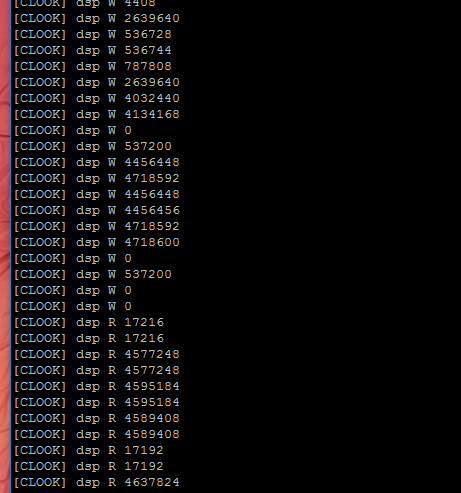
\includegraphics[scale=0.75]{clook_output}
                    \captionsetup{justification=centering}
                    \caption{Actual print statements from our CLOOK IO scheduler source code.}
                \end{figure}
        	\end{itemize}
    \end{itemize}
    
    
    \newpage
   
    \section*{Questions}
    \begin{enumerate}
        \item What do you think the main point of this assignment is?
        \begin{itemize}
            \item The main point of this assignment was to familiarize ourselves with the idea of I/O scheduling, as well as several methods of implementation. Beyond that, I think that this assignment is also designed to show us how to customize our kernel and run a virtual machine with different settings.
        \end{itemize}
        \item How did you personally approach the problem? Design decisions, algorithm, etc.
        \begin{itemize}
            \item Designing the algorithm for the solution to this project took a little abstract thinking and a lot of diagrams and notes. The first thing we did when assigned this was find the noop\_iosched.c and figure out what functions we could use, as well as what functions needed to be modified. The algorithm design was a bit more of a challenge, as it required extensive research and written out diagrams. Figuring out what files to modify to add C-LOOK to the I/O Scheduler List was also a bit convoluted and consisted of guessing and checking.
        \end{itemize}
        \item How did you ensure your solution was correct? Testing details, for instance.
        \begin{itemize}
            \item Checking if the implementation is correct was fairly simple. Once the virtual machine was up and running, we used the command \texttt{cat /sys/block/hda/queue/scheduler}. This returned the scheduler currently in use, which was [CLOOK]. Additionally, the running the kernel from the gdb printed out all of our debugging statements, regarding all the Read and Write requests which were being processed in CLOOK fashion (see Figure 1 above for details). 
        \end{itemize}
        \item What did you learn?
        \begin{itemize}
            \item This assignment led to some interesting discoveries. First and foremost, the project gave us a better understanding of I/O schedulers and the different methods of implementation. I think we gained a lot more insight and experience with I/O schedulers by actually writing one ourselves, as apposed to just reading about it. This project also exemplified how to customize the kernel before running the virtual machine. Finally, we learned that certain machine settings can be returned to the command line using the \texttt{cat} command.
        \end{itemize}
    \end{enumerate}
    
    
\end{document}
